\documentclass[11pt,letterpaper]{letter} % Specify the font size (10pt, 11pt and 12pt) and paper size (letterpaper, a4paper, etc)

\usepackage{graphicx} % Required for including pictures
\usepackage{microtype} % Improves typography
\usepackage{gfsdidot} % Use the GFS Didot font: http://www.tug.dk/FontCatalogue/gfsdidot/
\usepackage[T1]{fontenc} % Required for accented characters
\usepackage{lmodern}

% Create a new command for the horizontal rule in the document which allows thickness specification
\makeatletter
\def\vhrulefill#1{\leavevmode\leaders\hrule\@height#1\hfill \kern\z@}
\makeatother

%----------------------------------------------------------------------------------------
%	DOCUMENT MARGINS
%----------------------------------------------------------------------------------------

\textwidth 6.75in
\textheight 9.25in
\oddsidemargin -.25in
\evensidemargin -.25in
\topmargin -1in
\longindentation 0.50\textwidth
\parindent 0.4in

%----------------------------------------------------------------------------------------
%	SENDER INFORMATION
%----------------------------------------------------------------------------------------

\def\Who{Olalekan P. Ogunmolu} % Your name
\def\What{, PhD} % Your title
\def\Position{Postdoctoral Researcher} % Your position
\def\WhereOne{Perelman School of Medicine} % Your department/institution
\def\WhereTwo{University of Pennsylvania} % Your department/institution
\def\Address{3620 Hamilton Walk \\John Morgan Building - Room 183} % Your address
\def\CityZip{Philadelphia, PA 19104} % Your city, zip code, country, etc
\def\Email{ogunmolo@pennmedicine.upenn.edu} % Your email address
\def\TEL{Phone: (972) 375-6346} % Your phone number


%----------------------------------------------------------------------------------------
%	HEADER AND FROM ADDRESS STRUCTURE
%----------------------------------------------------------------------------------------

\address{
%\includegraphics[width=1in]{UC-Shield-full-color-LGE.jpg} % Include the logo of your institution

\includegraphics[width=1.1in]{PennShieldOnly.png} % Include the logo of your institution
\hspace{5.5in} % Position of the institution logo, increase to move left, decrease to move right
\vskip -1.07in~\\ % Position of the text in relation to the institution logo, increase to move down, decrease to move up
\Large\hspace{1.5in}THE UNIVERSITY \hfill ~\\[0.05in] % First line of institution name, adjust hspace if your logo is wide
\hspace{1.5in}OF PENNSYLVANIA \hfill \normalsize % Second line of institution name, adjust hspace if your logo is wide
\makebox[0ex][r]{\bf \Who \What }\hspace{0.08in} % Print your name and title with a little whitespace to the right
~\\[-0.11in] % Reduce the whitespace above the horizontal rule
\hspace{1.5in}\vhrulefill{1pt} \\ % Horizontal rule, adjust hspace if your logo is wide and \vhrulefill for the thickness of the rule
\hspace{\fill}\parbox[t]{2.85in}{ % Create a box for your details underneath the horizontal rule on the right
\footnotesize % Use a smaller font size for the details
\Who \What \\ \em % Your name, all text after this will be italicized
\Position\\ % Your title
\WhereOne\\ % Your department
\WhereTwo\\ % Your department
\Address\\ % Your address
\CityZip\\ % Your city and zip code
\TEL\\ % Your phone number
\Email\\ % Your email address
}
\hspace{-0.4in} % Horizontal position of this block, increase to move left, decrease to move right
\vspace{-1in} % Move the letter content up for a more compact look
}

%----------------------------------------------------------------------------------------
%	TO ADDRESS STRUCTURE
%----------------------------------------------------------------------------------------

\def\opening#1{\thispagestyle{empty}
{\centering\fromaddress \vspace{1in} \\ % Print the header and from address here, add whitespace to move date down
\hspace*{0.0in}\today\hspace*{\fill}\par} % Print today's date, remove \today to not display it
{\raggedright \toname \\ \toaddress \par} % Print the to name and address
\vspace{0.4in} % White space after the to address
\noindent #1 % Print the opening line
% Uncomment the 4 lines below to print a footnote with custom text
\def\thefootnote{}
\def\footnoterule{\hrule}
\footnotetext{\hspace*{\fill}{\footnotesize $\bullet$ \Who \hspace{.1em} $\bullet$ Penn Medicine \hspace{.1em} $\bullet$ Email: \Email \hspace{.1em} $\bullet$ \TEL \hspace{.1em} $\bullet$}}
\def\thefootnote{\arabic{footnote}}
}

%----------------------------------------------------------------------------------------
%	SIGNATURE STRUCTURE
%----------------------------------------------------------------------------------------

\signature{
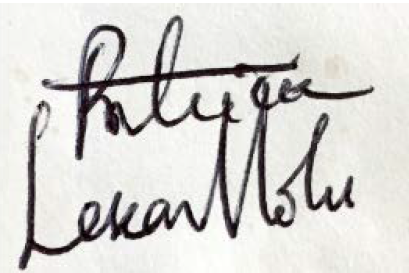
\includegraphics[width=1.4in]{signature.png}\\
\Who \What
}

\long\def\closing#1{
\vspace{0.2in} % Some whitespace after the letter content and before the signature
\noindent % Stop paragraph indentation
\hspace*{\longindentation} % Move the signature right
\parbox{\indentedwidth}{\raggedright
#1 % Print the signature text
\vskip 0.05in % Whitespace between the signature text and your name
\fromsig}} % Print your name and title

%----------------------------------------------------------------------------------------

\begin{document}

%----------------------------------------------------------------------------------------
%	TO ADDRESS
%----------------------------------------------------------------------------------------

\begin{letter}
	{\\
		 \textbf{Letter of Intent for Immigration Petition at USCIS} \\
	}
	
	%----------------------------------------------------------------------------------------
	%	LETTER CONTENT
	%----------------------------------------------------------------------------------------
	
%	\opening{Dear USCIS Officer,}
	\opening{}
	
	\vskip -0.87in~ \\
	
	\noindent\textbf{Background}: I am an interdisciplinary researcher who combines the scientific elegance of %scientific theory in 
	 machine learning and control theory with the practical impact of modern robotics to create technological solutions that improve healthcare delivery for cancer  patients. I am currently a postdoctoral researcher at The University of Pennsylvania's School of Medicine and I was previously a visiting postdoctorasl scholar at the University of Chicago's School of Medicine. In my postdoctoral research duties, I work on problems spanning conceptualization of new hardware  and software tools for improving the \textit{treatment planning} process in \textit{cancer radiation therapy} in our medical clinics at these Universities. My work has made meaningful impact in disciplines within and outside medicine, with citations from government and highered learning research institutions across the globe. Example institutions that have used my work include the National Aeronautics and Space Agency's Jet Propulsion Laboratory (NASA JPL), the 6th R\&D institute of South Korea's Agency for Defense Development, Uber AI Labs, and the Chinese Academy of Sciences among others.
	 
	\noindent\textbf{Future Research Plans}: My research in the past has focused on deriving the control and machine learning theoretical underpinnings for realizing my technical objectives namely using robots as motion-compensation systems during cancer radiation therapy. Going forward, my goal is to scale the use of the robots I have proposed and designed away from phantom tests to clinical trials at hospitals and medical schools in the United States, where I will have access to facilities to carry out my research. I want to achieve my goals in the United States because cancer is a large economic burden to the United States. This year alone, it is projected that 1,762,450 new cases of cancer will be diagnosed, and 606,880 people will die from the disease. This constitutes a national expenditure of 4.2\% of overall health care spending per 2017 budget. Along with the excellent researchers that I collaborate with at Penn Medicine, I am working on the next stages of deploying these robots on real-world cancer patients to help doctors, medical physicists, dosimetrists and lab clinicians better manage cancer treatments. 
	
	\noindent\textbf{Future Job Opportunites}: To realize my research objectives, I am being actively sought out for research opportunities at large research corporations in America. For example, on October 1st, a PhD recruiter at Facebook AI Research sought me out asking about my availability for a research opportunity  where I can apply my skills to solving real-world problems. Here is an excerpt from her email  \textit{``I saw your background and thought you would be a great addition to our team. Facebook has been rapidly growing and we are on the look-out for top PhD's/researchers to help our on our mission to give people the power to build community and bring the world closer together. As a PhD [sic], your research background would be considered since our aim is to find a team that aligns with your expertise and interests"}. I am also currently in the final stages of my interview process with Brandeis University in Massachusetts where I will be helping develop the next generation of roboticists as an instructor in robot manipulation, planning and control.
	
	\noindent\textbf{Conclusions}: Given my record of past successes at my research, and academic endeavors, I am confident in my ability to find a suitable job in the United States once I receive my Visa. I have responded to the challenges in my field with a novel and accurate robot motion-compensation system for real-time cancer irradiation on a treatment bed, while guaranteeing patient comfort, dose efficacy and providing compliance in manipulation -- conditions that other researchers' innovation have not met. I have a masters degree in control systems, which was very helpful when I started the head and neck immobilization project in RT during my PhD in robotics at the University of Texas at Dallas. My unique background has led me to a postdoc position at one of the finest medical schools in the country where I continue to combine scientific elegance with practical impact, delivering on technologies to advance the state of bleeding-edge healthcare in the United States. I intend to continue contributing to the research community while gaining dicipline expertise and helping develop the next generation of talents through mentorship programs.
	
	\closing{Sincerely,}
	
	%----------------------------------------------------------------------------------------
	
\end{letter}
\end{document}
